% ejersicios.tex
\section{Ejercicios}

\subsection{Ejercicio 1: Sistema Masa-Resorte-Amortiguador}

Resolver la ecuación diferencial que modela un sistema masa-resorte-amortiguador con $m = 2$ kg, $c = 8$ Ns/m, y $k = 32$ N/m, con condiciones iniciales $x(0) = 0.1$ m y $x'(0) = 0$ m/s.

\textbf{Solución:}
La ecuación diferencial es:
\begin{equation}
    2 \frac{d^2 x}{dt^2} + 8 \frac{dx}{dt} + 32x = 0
\end{equation}

Simplificando:
\begin{equation}
    \frac{d^2 x}{dt^2} + 4 \frac{dx}{dt} + 16x = 0
\end{equation}

La ecuación característica es:
\begin{equation}
    r^2 + 4r + 16 = 0
\end{equation}

Las raíces son: $r = -2 \pm 2\sqrt{3}i$

La solución general es:
\begin{equation}
    x(t) = e^{-2t} (C_1 \cos(2\sqrt{3}t) + C_2 \sin(2\sqrt{3}t))
\end{equation}

Aplicando las condiciones iniciales:
\begin{align}
    x(0) &= C_1 = 0.1 \\
    x'(0) &= -2C_1 + 2\sqrt{3}C_2 = 0 \Rightarrow C_2 = \frac{0.2}{2\sqrt{3}} = \frac{0.1}{\sqrt{3}}
\end{align}

La solución particular es:
\begin{equation}
    x(t) = e^{-2t} \left(0.1 \cos(2\sqrt{3}t) + \frac{0.1}{\sqrt{3}} \sin(2\sqrt{3}t)\right)
\end{equation}

\begin{figure}[H]
    \centering
    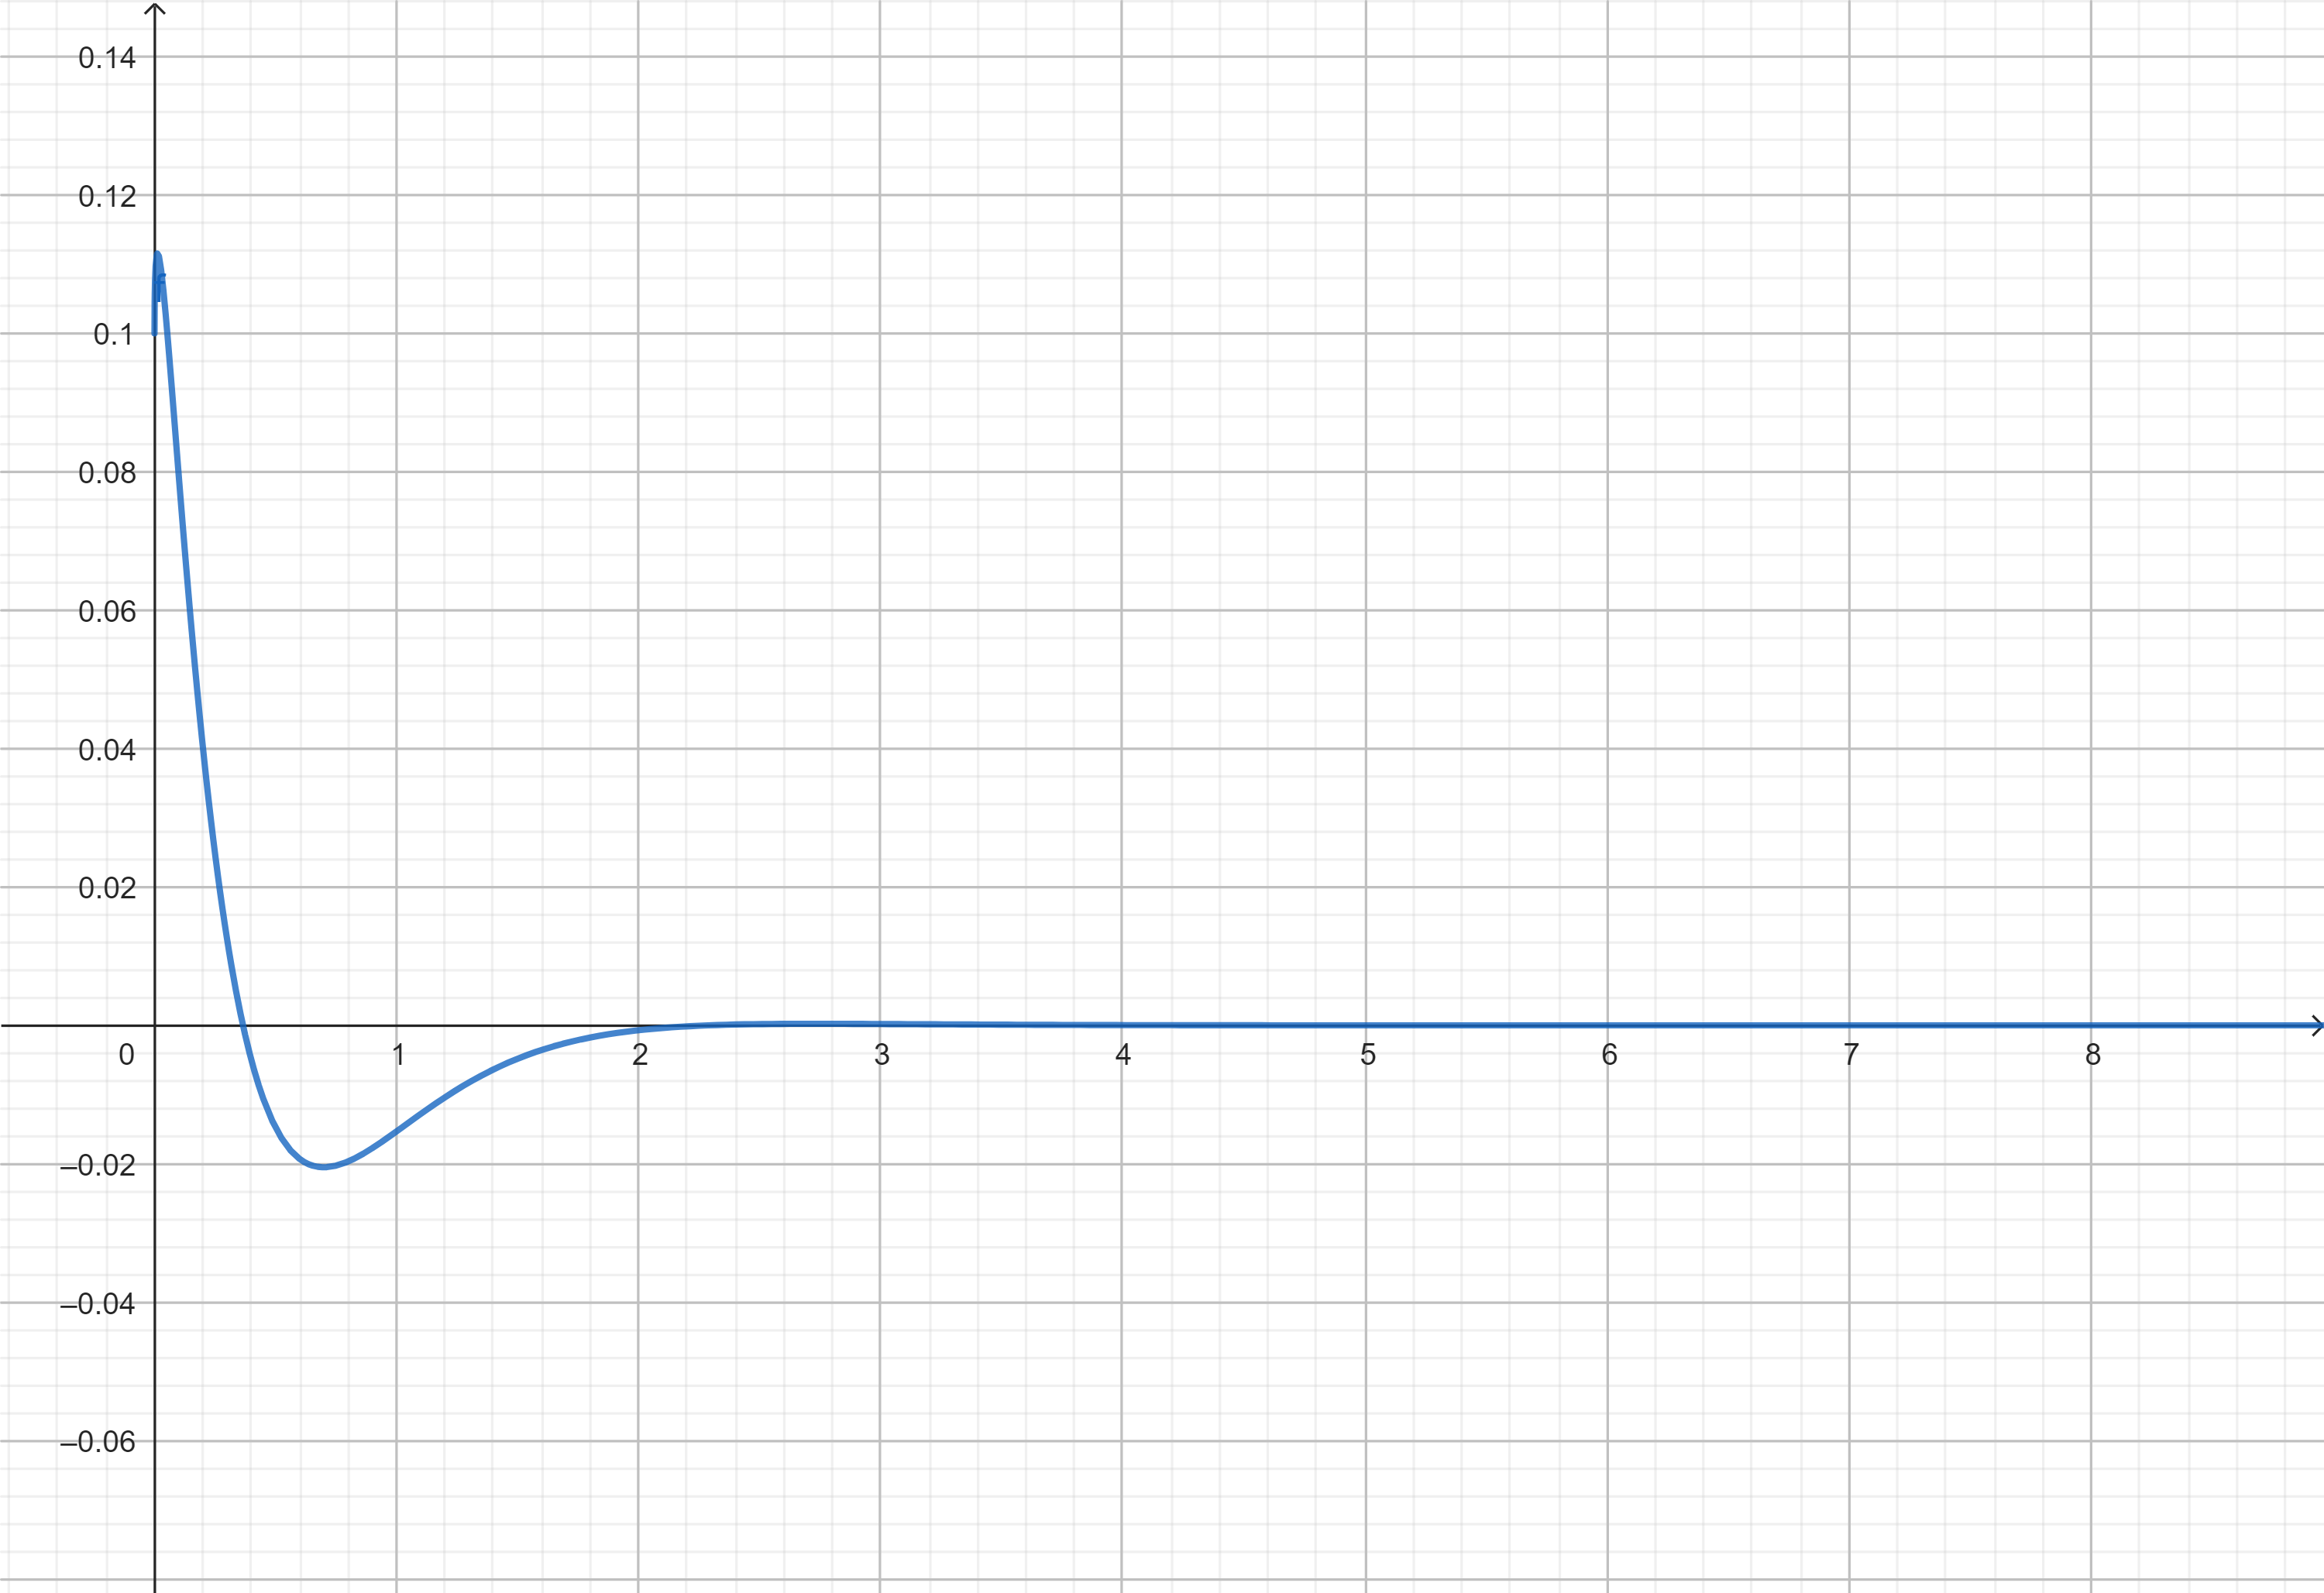
\includegraphics[width=0.8\textwidth]{imagen-ejercicio1.png}
    \caption{Respuesta temporal del sistema masa-resorte-amortiguador obtenida con GeoGebra}
\end{figure}

\subsection{Ejercicio 2: Circuito RLC en Serie}

Un circuito RLC en serie tiene $R = 100\ \Omega$, $L = 0.5$ H, y $C = 10\ \mu$F. Determinar la corriente $i(t)$ si la fuente de voltaje se retira repentinamente y $i(0) = 0.1$ A, $\frac{di}{dt}(0) = 0$.

\textbf{Solución:}
La ecuación del circuito es:
\begin{equation}
    L \frac{d^2 i}{dt^2} + R \frac{di}{dt} + \frac{1}{C} i = 0
\end{equation}

Sustituyendo valores:
\begin{equation}
    0.5 \frac{d^2 i}{dt^2} + 100 \frac{di}{dt} + 10^5 i = 0
\end{equation}

La ecuación característica es:
\begin{equation}
    0.5r^2 + 100r + 10^5 = 0
\end{equation}

Las raíces son: $r = -100 \pm 400i$

La solución es:
\begin{equation}
    i(t) = e^{-100t} (C_1 \cos(400t) + C_2 \sin(400t))
\end{equation}

Aplicando condiciones iniciales:
\begin{align}
    i(0) &= C_1 = 0.1 \\
    \frac{di}{dt}(0) &= -100C_1 + 400C_2 = 0 \Rightarrow C_2 = 0.025
\end{align}
\begin{figure}[H]
    \centering
    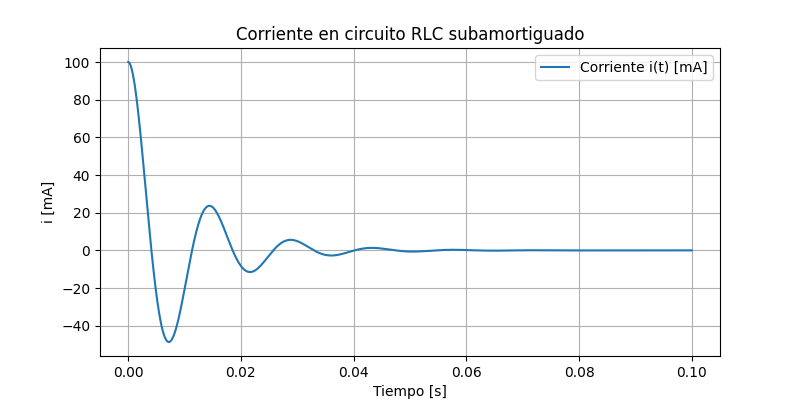
\includegraphics[width=0.8\textwidth]{imagen-ejercicio2.png}
    \caption{Corriente en el circuito RLC obtenida mediante simulación en Python}
\end{figure}

\subsection{Ejercicio 3: Sistema de Control de Nivel}

Un tanque de almacenamiento tiene una dinámica descrita por:
\begin{equation}
    A \frac{dh}{dt} = -k h
\end{equation}

donde $A = 5$ m² es el área transversal y $k = 0.5$ m²/s es el coeficiente de salida. Resolver para $h(t)$ con $h(0) = 2$ m.

\textbf{Solución:}
La ecuación se simplifica a:
\begin{equation}
    \frac{dh}{dt} + \frac{k}{A} h = 0
\end{equation}

Esta es una ecuación de primer orden homogénea con solución:
\begin{equation}
    h(t) = h(0) e^{-\frac{k}{A}t} = 2 e^{-0.1t}
\end{equation}

\begin{figure}[H]
    \centering
    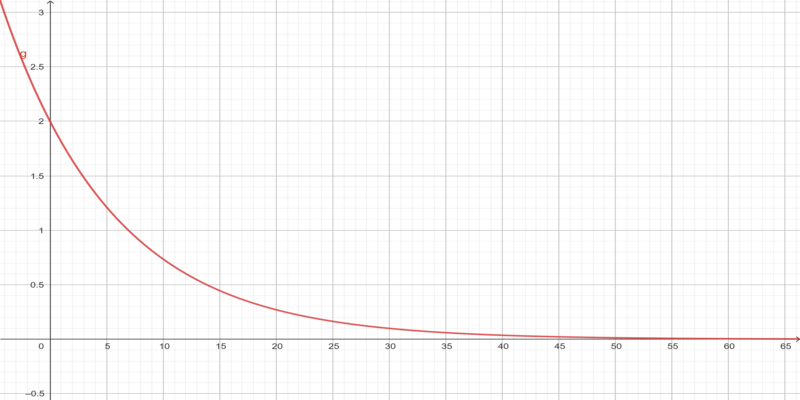
\includegraphics[width=0.8\textwidth]{imagen-ejercicio3.png}
    \caption{Nivel del tanque versus tiempo, simulado en GeoGebra}
\end{figure}

\subsection{Ejercicio 4: Modelo de Población con Migración}

La población de una ciudad cambia según:
\begin{equation}
    \frac{dP}{dt} = -\lambda P
\end{equation}

con $\lambda = 0.05\ \text{año}^{-1}$ y $P(0) = 100,000$. Determinar cuando la población se reduce a la mitad.

\textbf{Solución:}
La solución es:
\begin{equation}
    P(t) = 100,000 e^{-0.05t}
\end{equation}

Para $P(t) = 50,000$:
\begin{equation}
    50,000 = 100,000 e^{-0.05t} \Rightarrow t = \frac{\ln(0.5)}{-0.05} \approx 13.86 \text{ años}
\end{equation}

\begin{figure}[H]
    \centering
    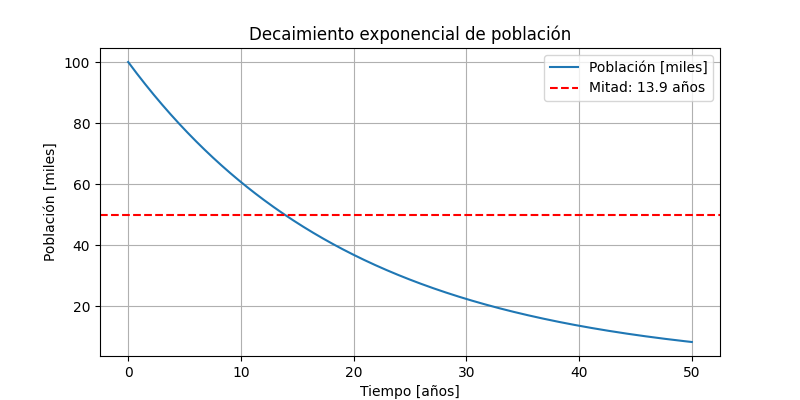
\includegraphics[width=0.8\textwidth]{imagen-ejercicio4.png}
    \caption{Decaimiento exponencial de la población modelado en Python}
\end{figure}

\subsection{Ejercicio 5: Sistema de Segundo Orden Sobreamortiguado}

Resolver:
\begin{equation}
    \frac{d^2 y}{dt^2} + 6 \frac{dy}{dt} + 8y = 0
\end{equation}

con $y(0) = 1$ y $y'(0) = 0$.

\textbf{Solución:}
La ecuación característica es:
\begin{equation}
    r^2 + 6r + 8 = 0
\end{equation}

Las raíces son: $r_1 = -2$, $r_2 = -4$

La solución general es:
\begin{equation}
    y(t) = C_1 e^{-2t} + C_2 e^{-4t}
\end{equation}

Aplicando condiciones iniciales:
\begin{align}
    y(0) &= C_1 + C_2 = 1 \\
    y'(0) &= -2C_1 - 4C_2 = 0
\end{align}

Resolviendo: $C_1 = 2$, $C_2 = -1$

La solución es:
\begin{equation}
    y(t) = 2e^{-2t} - e^{-4t}
\end{equation}

\begin{figure}[H]
    \centering
    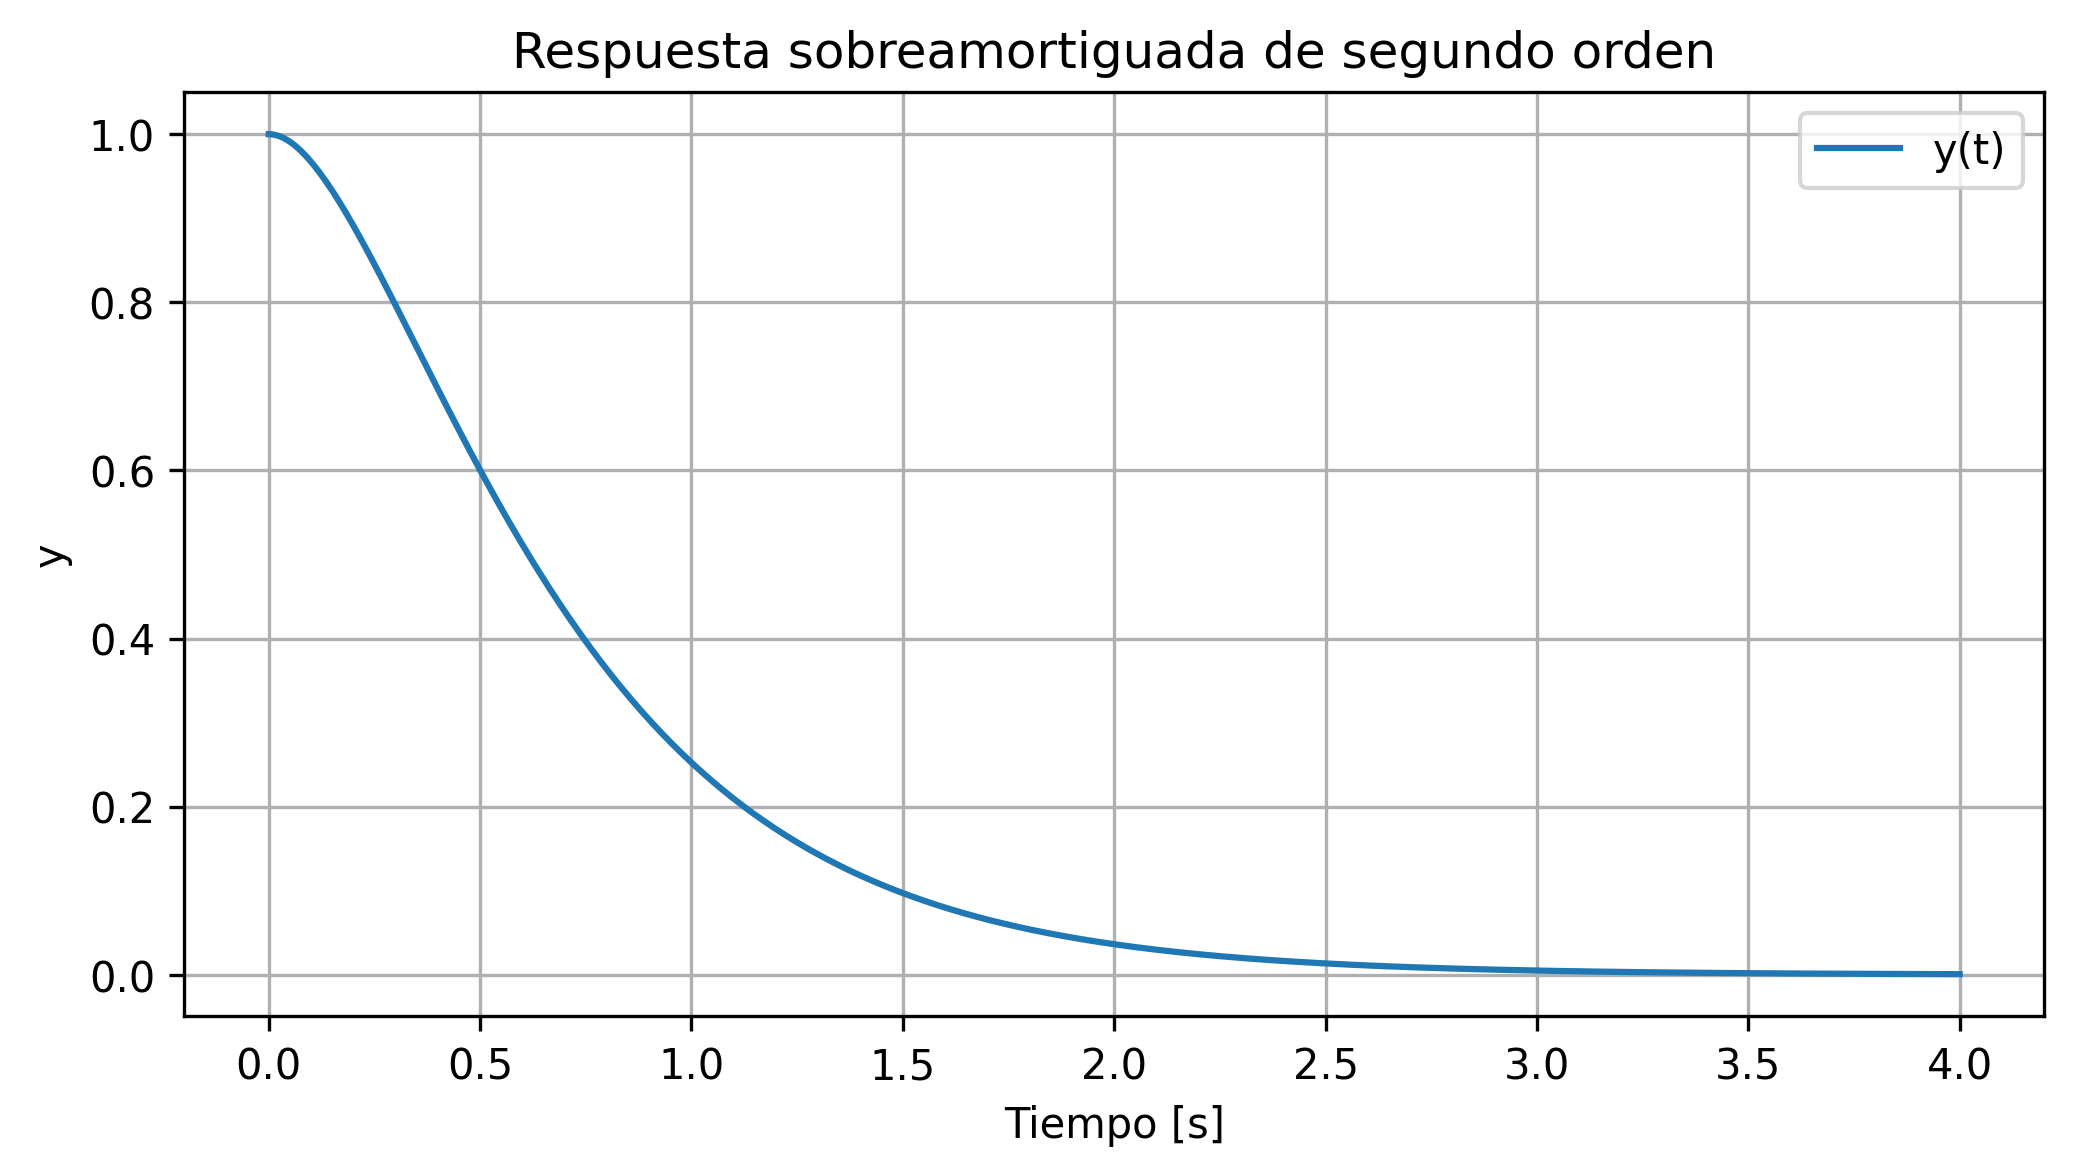
\includegraphics[width=0.8\textwidth]{imagen-ejercicio5.png}
    \caption{Respuesta sobreamortiguada del sistema de segundo orden, simulado en GeoGebra}
\end{figure}